\section{Measurement efficiency}

If scattered photons are lost through absorption, or if the parametric or HEMT amplifiers add noise to the scattered signal, the measurement performance degrades.
We characterized these imperfections by comparing the effect of the measurement photons on the qubit against the resulting measurement visibility.

In Chapter \ref{ch:DispersiveMeasurement} we found a relation between the measurement SNR, and the associated qubit dephasing.
For a given measurement pulse power, if the measurement visibility is less than that predicted by Eq.\,(\ref{eq:sec:measurementInducedDephasing:measurementInducedDephasing}), we would conclude that some of the scattered photons must have been lost, or additional noise must have been injected into the processing chain.
In one experiment, we measured the photon induced qubit dephasing via Ramsey fringes, where we added a variable power measurement pulse between the usual two $\pi$-pulses in the standard Ramsey sequence.
This measurement pulse dephases the qubit and lowers the visibility of the Ramsey fringes.
We record the resulting fringe visibility as a function of measurement pulse power.
In a second experiment, we prepare the qubit in either $\ket{0}$ or $\ket{1}$ and then apply a measurement pulse, recording the SNR as a function of pulse power.
We then convert SNR to an upper bound on phase coherence via Eq.\,(\ref{eq:sec:measurementInducedDephasing:measurementInducedDephasing}).

We extract the system efficiency by comparing the directly measured Ramsey visibility against the quantum limit implied from the second experiment, as shown in Fig.\,\ref{Fig:sec:measurementEfficiency:measurementEfficiency}.
We found that the Ramsey visibility curve is shifted 9\,dB to the left of the quantum limit curve, indicating that our measurement system has a quantum efficiency of $\eta=-9\,\text{dB} \approx 12\%$.

Quantum efficiency less than 1 comes from photon loss and/or added noise, so we attempt to budget this -9\,dB efficiency in terms of lossy hardware elements and known noise sources in the experiment.
At least 3\,dB efficiency loss comes from the parametric amplifier, as a phase insensitive parametric amplifier adds an input referred noise of $\hbar \omega_r/2$ noise power per unit bandwidth \cite{Caves:amplifiers1982}.
The photon states themselves carry $\hbar \omega_r / 2$ quantum noise power per unit bandwidth, so the parametric amplifier degrades the signal to noise ratio by at least a factor of $2 = 3\,\text{dB}$.

The remaining $6\,\text{dB}$ must come from a combination of other noise sources and photon loss.
Referring back to the diagram of the experimental apparatus shown in Fig.\,\ref{Fig:wiring}, we find a large number of microwave elements, each of which contributes some loss.
The IR filter itself is known to have approximately 2\,dB loss at our measurement frequencies near $7\,\text{GHz}$.
The three circulators are expected to contribute a total of $\sim$1\,dB loss.
The dispersed signal makes roughly 20 trips through SMA connectors.
With 0.03\,dB specified insertion loss per SMA connector, assuming the insertion loss really is a loss, the connectors contribute at least another 0.5\,dB loss.
The HEMT amplifier adds noise.
We operated with parametric amplifier gain near 16\,dB, which results in an effective output noise temperature of $T = 10^{16/10} h\nu / k_b \approx 13\,\text{Kelvin}$.
This is about 5 times higher than the HEMT noise temperature of $\sim$2.5 Kelvin, resulting in another 1\,dB of noise added by the HEMT.

With these considerations we have approximately 1.5\,dB loss or added noise unaccounted for, which corresponds to 70\% efficiency.
This extra efficiency loss could be carefully studied in further experiments.

Without precise measurements of the loss of each hardware element, it is difficult to estimate the uncertainty of the numbers discussed above.
However, the SMA connectors deserve special attention.
The insertion loss of an SMA connector does not necessarily come from a dissipative processes; non-zero reflections from the input contribute to insertion loss.
Therefore, our assumption that the collective insertion losses of the 20 SMA connectors add together is not necessarily well founded.
Ignoring the SMA connector insertion loss, we compute 2.0\,dB loss or added noise unaccounted for.


\begin{figure}
\begin{centering}
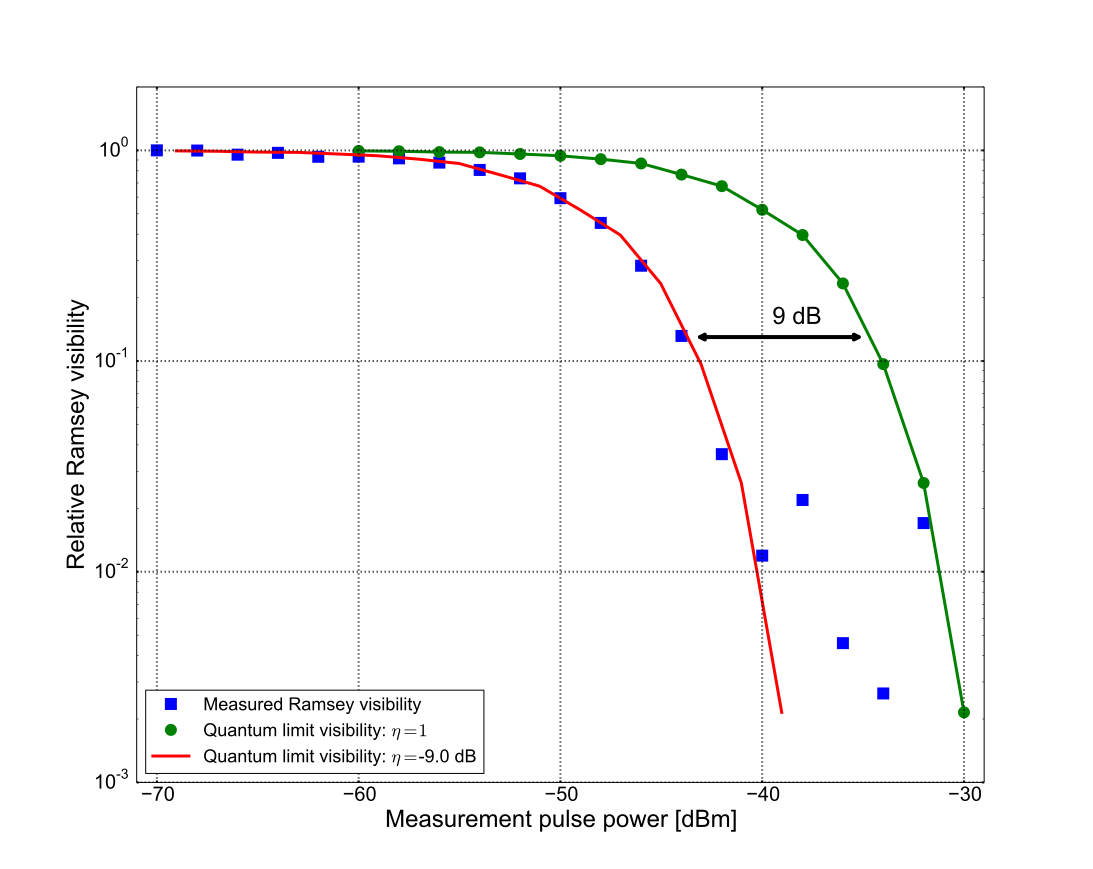
\includegraphics[width=\textwidth]{measurementEfficiency.pdf}
\par\end{centering}
\caption{Quantum efficiency of the measurement system. Performing a standard Ramsey fringe sequence, but with a measure pulse in between the $\pi/2$-pulses, we measure the relative fringe visibility as a function of measure pulse power (blue squares). The fringe visibility data becomes noisy at visibilities $<3\%$. We also measure the distinguishability between the qubit states versus measure pulse power, and convert to a quantum limit on Ramsey fringe visibility via Eq.\,(\ref{eq:sec:measurementInducedDephasing:measurementInducedDephasing}) (green circles). The comparison between these curves is clarified by re-plotting the quantum limit shifted by 9\,dB (red line), which goes through the Ramsey visibility points.}
\label{Fig:sec:measurementEfficiency:measurementEfficiency}
\end{figure}
